\documentclass[a4paper,twoside]{article}

\usepackage{microtype}
\usepackage{epsfig}
\usepackage{subcaption}
\usepackage{calc}
\usepackage{amssymb}
\usepackage{amstext}
\usepackage{amsmath}
\usepackage{amsthm}
\usepackage{multicol}
\usepackage{pslatex}
\usepackage{apalike}
\usepackage{csquotes}
\usepackage[hidelinks]{hyperref}
\usepackage{cleveref}
\usepackage{numprint}
\usepackage{SCITEPRESS} 
\usepackage{flushend}

\usepackage{tikz}
\usetikzlibrary{calc,positioning,spy}

\usepackage{booktabs}

\usepackage{float}
\newfloat{lstfloat}{htbp}{lop}
\floatname{lstfloat}{Listing}

\usepackage[nolist]{acronym}


\usepackage{listings} 
\usepackage{accsupp}


% This ensures numbers are not copied, but leading spaces are copied, as taken from
% http://tex.stackexchange.com/a/30310

\newcommand{\noncopynumber}[1]{%
    \BeginAccSupp{method=escape,ActualText={}}%
    #1%
    \EndAccSupp{}%
}

\makeatletter
\def\lst@outputspace{{\ifx\lst@bkgcolor\empty\color{white}\else\lst@bkgcolor\fi\lst@visiblespace}}
\makeatother


\definecolor{msvc_keyword}   {HTML}{0000FF} 
\definecolor{msvc_comment}   {HTML}{008000} 
\definecolor{msvc_background}{HTML}{eff0f1} 
\definecolor{msvc_frame}     {HTML}{000000}
\definecolor{msvc_linenumber}{HTML}{808080}
\definecolor{msvc_string}    {HTML}{000000}

\definecolor{msvc_directives}{HTML}{808080}
\definecolor{msvc_operators} {HTML}{000000}
\definecolor{msvc_stl}       {HTML}{000000}


\lstdefinelanguage{TypeScript}
{
    keywords        = {break, case, catch, continue, debugger, default, delete, do, else, finally, for, function, if, in, instanceof, new, return, switch, throw, try, typeof, var, void, while, with, super, class, constructor},
    morecomment     = [l]{//},
    morecomment     = [s]{/*}{*/},
    morestring      = [b]',
    morestring      = [b]", 
    keywordstyle    = \color{blue}\bfseries,
    identifierstyle = \color{black},
    commentstyle    = \color{teal}\ttfamily,
    stringstyle     = \color{red}\ttfamily,
    sensitive       = true,
    style           = TypeScript
}


\lstdefinestyle{TypeScript}
{
    basicstyle       = 
\linespread{0.85}\ttfamily
\lst@ifdisplaystyle\scriptsize\fi %inline code should have normal font size
%
,   backgroundcolor  = \color{msvc_background}
,   rulecolor        = \color{msvc_frame}
,   keywordstyle     = \lst@ifdisplaystyle\color{msvc_keyword}\fi
,   commentstyle     = \lst@ifdisplaystyle\color{msvc_comment}\fi
,   stringstyle      = \lst@ifdisplaystyle\color{msvc_string}\fi
,   showstringspaces = false
,   numberbychapter  = true
,   numbersep        =  8pt
,   showlines        = true
,   tabsize          =  2          
,   numbers          = left
,   numberstyle      = \tiny\color{msvc_linenumber}\noncopynumber
,   framesep         =  4pt
,   xleftmargin      = \parindent
,   xleftmargin      = 16pt
,   framexleftmargin = 16pt
,   abovecaptionskip = \medskipamount
,   stepnumber       = 1
,   columns          = flexible
,   keepspaces       = true
,	keywords         = [2]{ prototype, this }
,	keywordstyle     = [2]\lst@ifdisplaystyle\color{msvc_stl}\fi
,   morekeywords     = [1]{ noexcept }
,	literate         = *
{[}{{\lst@ifdisplaystyle\color{msvc_operators}\fi{[}}}{1}
{]}{{\lst@ifdisplaystyle\color{msvc_operators}\fi{]}}}{1}
}


\begin{document}
\title{Software Forest: A Visualization of Semantic Similarities\\in Source Code using a Tree Metaphor}

\author{
\authorname{Daniel Atzberger\sup{1},
    Tim Cech\sup{2},
    Merlin de la Haye\sup{2},
    Maximilian Söchting\sup{2},\\
    Willy Scheibel\sup{1},
    Daniel Limberger\sup{1},
    and Jürgen Döllner\sup{1}}
    \affiliation{Hasso Plattner Institute, Digital Engineering Faculty, University of Potsdam, Germany}
    \email{\sup{1}\{daniel.atzberger,
    willy.scheibel,
    daniel.limberger,
    juergen.doellner\}@hpi.de
    \\
    \sup{2}\{tim.cech,
    merlin.haye,
    maximilian.soechting\}@student.hpi.de
}
}

\keywords{Topic Modeling, Software Visualization, Source Code Mining}

\abstract{%
Software visualization techniques provide effective means for program comprehension tasks as they allow developers to interactively explore large code bases.
A frequently encountered task during software development is the detection of source code files of similar semantic.
To assist this task we present \emph{Software Forest}, a novel 2.5D software visualization that enables interactive exploration of semantic similarities within a software system, illustrated as a forest.
The underlying layout results from the analysis of the vocabulary of the software documents using Latent Dirichlet Allocation and Multidimensional Scaling and therefore reflects the semantic similarity between source code files.
By mapping properties of a software entity, e.g., size metrics or trend data, to visual variables encoded by various, figurative tree meshes, aspects of a software system can be displayed.
This concept is complemented with implementation details as well as a discussion on applications.
}

\onecolumn \maketitle \normalsize \setcounter{footnote}{0} \vfill

\section{\uppercase{Introduction}}
\label{sec:introduction}
\noindent
Program comprehension is of fundamental importance during the entire software development process, especially in the maintenance phase.
Getting a quick overview over a program's structure and functionalities is necessary for further development.
A question developers frequently encounter is whether there are already source code units of certain semantics in terms of features, concerns, and techniques. 
The identification of such code units can support decisions on feature location, encapsulation, and module architecture. 
Furthermore, this information helps to identify associated developers and could be used to, e.g., determine and assign reviewers.
This is a particular challenge for historically grown legacy systems, systems developed from distributed teams, or systems depending on a large technology stack.
In addition, the folder structure of a software project may deviate from its conceptual content over time.
Various software visualization techniques support developers by providing expressive images whose layouts are inspired by maps known from daily life.
They promote shared mental images that enable users to communicate more precisely and gain insight into abstract data.

\begin{figure}
    \centering

    \begin{tikzpicture}[spy using outlines={white, circle, magnification=2.5, size=80, connect spies, every spy on node/.append style={thin}}]
        \node[anchor=center, inner sep=0pt, outer sep=0pt](teaser) {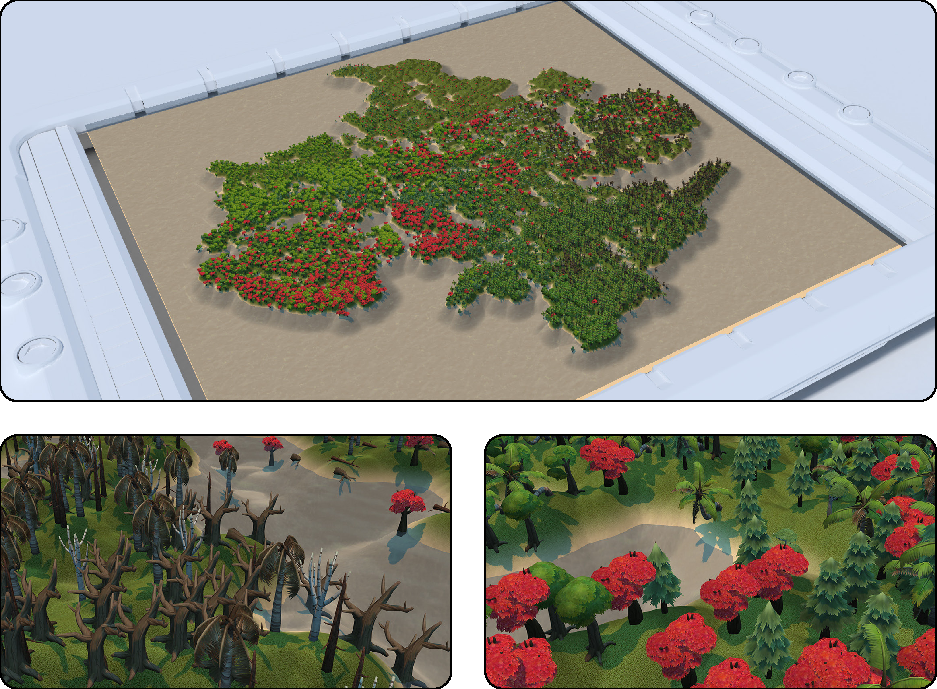
\includegraphics[width=\linewidth]{forest-teaser}};%
    \end{tikzpicture}
    \caption{A software forest depicting \numprint{11291} source code units (top). Each unit is positioned based on its semantic similarity w.r.t. to all other units. The unit's dominant topic is represented by the type of the tree (right, e.g., palm tree, deciduous tree, conifer) and additional attributes are be mapped to, e.g., tree health and tree growth (left).}
    \label{fig:teaser}

\end{figure}

\begin{figure*}[t]
    \centering
    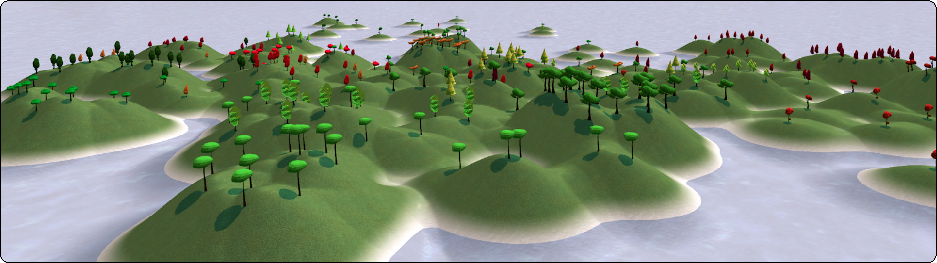
\includegraphics[width=\textwidth]{forest-microsoft}
    \caption{Visualization of the Microsoft Calculator open-source project in our framework. Tree types are chosen based on the topics, i.e., source code files with the same dominant topics are represented through the same tree type. Clusters of identical tree types, i.e., source code files with identical dominant topics, can be easily recognized in this example.}
    \label{fig:example1}
\end{figure*}

We present \emph{Software Forest}, a novel 2.5D software visualization technique for displaying semantic similarity of source code units.
The semantic content of software files is described as distributions over latent topics hidden in the source code by applying \ac{LDA}.
\ac{MDS} is used to compute a layout, where the distance of points reflect their semantic similarity.
Using a tree metaphor, \emph{Software Forest} introduces various visual variables for topic emphasis and additional data display, e.g., software metrics, and offers possibilities for displaying static as well as evolutionary data~(\autoref{fig:teaser}).
The following contributions are made:
\begin{enumerate}
    \item We present a layout algorithm based on the application of \ac{LDA} and \ac{MDS} on source code files, thereby mirroring the semantic relatedness of documents such as source code units.
    \item We enlist and review visual variables inherent to the tree metaphor and discuss possibilities and applications for software visualization tasks.
    \item We provide technical notes on the implementation of our visualization, discuss its features and limitations, and provide a web-based prototype for interactive exploration and evaluation.
\end{enumerate}

The remainder of this paper is organized as follows.
\Cref{sec:related work} discusses background and related work.
In \Cref{sec:layout}, we detail our layout algorithm.
\Cref{sec:conceptvisualization} presents our visualization concept using visual variables of trees (figuratively).
\Cref{sec:implementation} highlights implementation aspects regarding the data processing pipeline and the visualization framework.
\Cref{sec:results} discusses application scenarios and limitations of the current approach.
\Cref{sec:conclusion} concludes this paper and outlines direction for future work.

\section{\uppercase{Related Work}}
\label{sec:related work}
\noindent
Related work is mainly identified in two research areas: (1) preprocessing of software system data by means of topic extraction and dimension reduction and (2) thematic maps, map-based visualizations, and visualization metaphors in general. 

\paragraph{Data Processing.}
Since a large part of a developer's knowledge of the project is directly encoded in the source code through comments and identifier names, a layout origin from the vocabulary could reflect the project's semantic structure.
This approach was pursued for the first time by Kuhn et~al. \cite{kuhn2008consistentlayout}.
They examine the natural language found in source code to generate software visualization.
In a first stage source files are parsed and a term-document-matrix is created, which stores the frequency of each word in a document.
The high-dimensional document-word-vectors, i.e., the columns of the term-document-matrix, are projected to the plane by applying \ac{LSI} \cite{deerwester1990indexing} followed by \ac{MDS} \cite{cox2008multidimensional}.
By creating a height field which represents the LOC, island-like landscapes are created which allow semantic affiliations to be deduced.
Another visualization of natural language texts, which utilizes a cartographic metaphor, can be found in \cite{skupin2004worldofgeography}.
The layout, which is created by using a self-organizing map \cite{kohonen1997som} on the term-document-matrix, is enriched with a height field.
In their investigations the authors limit themselves to abstracts from publications of the geographic domain.
For the visualization of source code this can be extended by suitable preprocessing.

The main difference between our work and the previously presented is that our layout is based on a probabilistic topic model, \ac{LDA} specifically.
It is known that the pure \ac{BOW} model is not able to recognize synonymy and polysemy.
Although \ac{LSI} can recognize synonyms, polysemy is still an issue.
Probabilistic models, e.g., \ac{LDA} can help to overcome both problems.
Besides the layout, we can also map properties of the topic distribution to visual variables of the trees (\autoref{fig:example1}).
Since \ac{LDA} has been used for numerous software mining tasks, it is not surprising that the obtained results were represented by dimension reductions.
For instance, Linstead et~al. used LDA and the author-topic model \cite{rosen-zvi2004authors} to detect semantic similarity between documents and developers \cite{linstead09sourcerer}.
The resulting document-topic distributions are displayed by applying \ac{MDS} to reduce them to two dimensions.
Nevertheless, this neglects the fact that the similarity between topics among each other might differ.
We circumvent this issue by first applying a dimension reduction to the topic distributions and then aggregating the document vectors as linear combinations.

Another problem which adresses the question of positionining elements in a way that reflects their semantic similarity was presented in \cite{barth2014semantic}.
Barth et~al. presented three novel layout algorithms for word clouds, where the distance between the words should capture their semantic relatedness.
Our considerations neglect the similarity of words and address the representation of semantic similarity of documents.

\paragraph{Visualization Metaphors.}

A majority of the underlying layouts of software visualizations are based on the hierarchical folder structure \cite{holten2005,bundleview}.
Treemaps are a widely used technique in hierarchy visualization \cite{scheibel2020-treemaptaxonomy} and are prominently used for software visualization as they provide a wide variety of visual variables \cite{limberger2019-softwaremap}.

Besides classic visual variables like block height, texture or color a 2.5D treemap offers creative ways for visualizing dynamic properties of a software system.
An example is presented by W{\"u}rfel et~al., who showed how natural phenomena such as fire and rain can be used to visualize the evolution of source code artifacts \cite{wurfel2015natural}.
In this context, \emph{CodeCity} \cite{Wettel2007SoftwareCities} and the \emph{Software City} \cite{steinbruckner2013-evolution} are well known metaphors.
By mapping source code metrics, e.g., \ac{LOC}, to visual variables of cuboids, e.g., the height, visualizations are created, which remind optically of modern cities.
The approach was further developed in later work and integrated into IDEs \cite{balogh2015-codemetropolis}.
Next to rectangular layouts, map-like shapes are used in hierarchy visualization as well \cite{auber2013-gospermap}.
With focus on software visualization, the map metaphor is extended to derive layouts from dependencies \cite{hawes2015-codesurveyor}.
The map metaphor is further used in conjunction with oceans and islands that are derived from Voronoi diagrams \cite{schreiber2018-islandmetaphor}.
Another approach for visualizing software metrics inspired by nature are \emph{Software Feathers}, a visualization approach for object-oriented entities like classes and interfaces with feathers \cite{beck2014-feathers}.
The structure of feathers is determined by numerous parameters, e.g., their size, shape, or texture, which provides many possible mappings of software metrics.
Similar to our forest and landscape visualization, \u{S}t\u{e}p\'{a}nek proposes a visualization primarily composed of trees, wood cabins and islands \cite{stepanek2020-landscapesthesis}.
The layout of source code units is calculated based on a weighted graph, with files that reference each other having a stronger pull toward one another.
Different file types are represented with different metaphors, e.g., classes are represented with trees while value types (structs) are visualized using small cabins.

Kleiberg et~al. proposed another visualization which mainly bases on the tree metaphor \cite{kleiberg2001botanical}.
The authors generate a botanic tree whose branches and fruits display hierarchical structures.
Our work completely neglects the underlying hierarchical structure of a software system provided by its folder structure.
Additionaly a single tree is used to display a single file rather than an entire project.

\section{\uppercase{Layout Computation}}
\label{sec:layout}
\noindent
The underlying layout of a software forest is constructed to reflect the semantic similarity of the source code units, in our case files contained in a source code repository.
Thus, we analyze the use of natural language in the source code.
We first preprocess the corpus $\mathcal{C} = \{ d_1, \dots, d_m \}$ of software files $d_1, \dots, d_m$ to get rid of the words in the vocabulary that do not carry a semantic meaning.
We then compute a formal description of the documents as distributions over latent topics using \ac{LDA}.
The resulting high-dimensional vectors describing topics are reduced by \ac{MDS} to two components, which finally aggregate to the positions of document vectors.

\begin{table*}[t]
    \footnotesize
    \centering
	\setlength{\tabcolsep}{10.0pt}%
	\renewcommand{\arraystretch}{1.05}
    \begin{tabular}{c|c||c|c||c|c}
    \toprule
    \multicolumn{2}{c||}{\textbf{Topic \#1}} & \multicolumn{2}{c||}{\textbf{Topic \#2}} & \multicolumn{2}{c}{\textbf{Topic \#3}} \\ \midrule
    \textbf{Term} & \textbf{Probability} &
    \textbf{Term} & \textbf{Probability} & \textbf{Term} & \textbf{Probability}\\ \midrule
         std & 0.070 & thread & 0.132 & address & 0.115 \\
         transaction & 0.031 & time & 0.070 & model & 0.108 \\
         fee & 0.027 & queue & 0.064 & table & 0.065 \\
        tx & 0.026 & std & 0.054 & label & 0.051\\
        ban & 0.024 & callback & 0.040 & qt & 0.033\\
        str & 0.023 & run & 0.037 & index & 0.030 \\
        handler & 0.016 & call & 0.025 & dialog & 0.024 \\
        output & 0.016 & mutex & 0.021 & column & 0.024\\
        bitcoin & 0.015 & scheduler & 0.020 & ui & 0.021 \\
        reason & 0.015 & wait & 0.018 & role & 0.019 \\ \hline
    \end{tabular}
    \caption{Three exemplary topics extracted from \emph{Bitcoin Core} (\href{https://github.com/bitcoin/bitcoin}{github.com/bitcoin/bitcoin}) source code with $K = 50$.}
    \label{tab:topics_bitcoin}
\end{table*}

\subsection{Preprocessing Data}
Although source code resembles natural language in its vocabulary, various preprocessing steps are required to get rid of words that do not carry relevant semantic meaning. 
For this, we implement an algorithm, processing all documents as follows:
\begin{description}

    \item [1. Removal of Non-text Symbols:] All special characters such as dots and semicolons are replaced with white spaces to avoid accidental connection of words not meant to be combined.
    This includes the splitting of identifier names, e.g., the word \emph{foo.bar} gets split into \emph{foo} and \emph{bar}.
    
    \item [2. Split of Words:] Identifiers are split according to delimiters and the camel case convention, e.g., \emph{FooBar} is split into \emph{foo} and \emph{bar}, and stripped from redundant white space subsequently. 

    \item [3. Removal of Stop Words:] Stop words based on natural language and keywords of programming language are removed as they carry no semantic content. Additionally, we filter the input based on a hand-crafted list comprising domain specific stop words, data types, type abstractions etc.
    
    \item [4. Lemmatization:] To avoid grammatical diversions, all words are reduced to their basic form, e.g., \emph{said} and \emph{saying} are reduced to \emph{say}.

\end{description}

After preprocessing, we store all documents as \ac{BOW}, i.e., the order in which the words occur is neglected and only their frequency is stored.
We are not introducing new identifiers for this notation and, when using the term \emph{documents}, always refer to their representation as \ac{BOW}.
The term-document-matrix stores these \ac{BOW} vectors as its columns.

\subsection{Latent Dirichlet Allocation}
Given a corpus $\mathcal{C} = \{d_1, \dots, d_m \}$ of documents that share a vocabulary $\mathcal{V} = \{w_1, \dots, w_N\}$, a probabilistic topic model extracts semantic clusters in its vocabulary, so-called \emph{topics}, as multinomial distributions over the vocabulary $\mathcal{V}$.
Additionally each document is described as a mixture of the extracted topics, which describe its document's semantic structure.
Given a number $K$ of topics specified as a hyperparameter together with Dirichlet priors $\alpha = (\alpha_1, \dots, \alpha_K)$, where $\alpha_i > 0$ for all $1\le i \le K$ and $\beta = (\beta_1, \dots, \beta_N)$, where $\beta_j > 0$ for all $1 \le j \le N$ that capture the document-topic-distributions and the topic-term-distribution respectively, \ac{LDA} defines a fully generative model for the creation of a corpus \cite{blei2003latent}.
The generation process for a document $d$ operates as follows:
\begin{enumerate}
    \item choose a distribution over topics $\theta \sim \text{Dirichlet}(\alpha)$
    \item for each word $w$ in $d$
    \begin{enumerate}
        \item choose a topic $z \sim \text{Multinomial}(\theta)$
        \item choose the word $w$ according to the probability $p(w \vert z, \beta)$
    \end{enumerate}
\end{enumerate}

\autoref{tab:topics_bitcoin} exemplarily shows the top 10 words of 3 manually selected topics applied on the corpus derived from the source code of the \emph{Bitcoin Core}.
These often suggest the concept underlying the topic, e.g., the third topic covers user interaction.
The number of topics was chosen such that the extracted topics were easily interpretable by humans.

\begin{figure}[b]
    \centering
    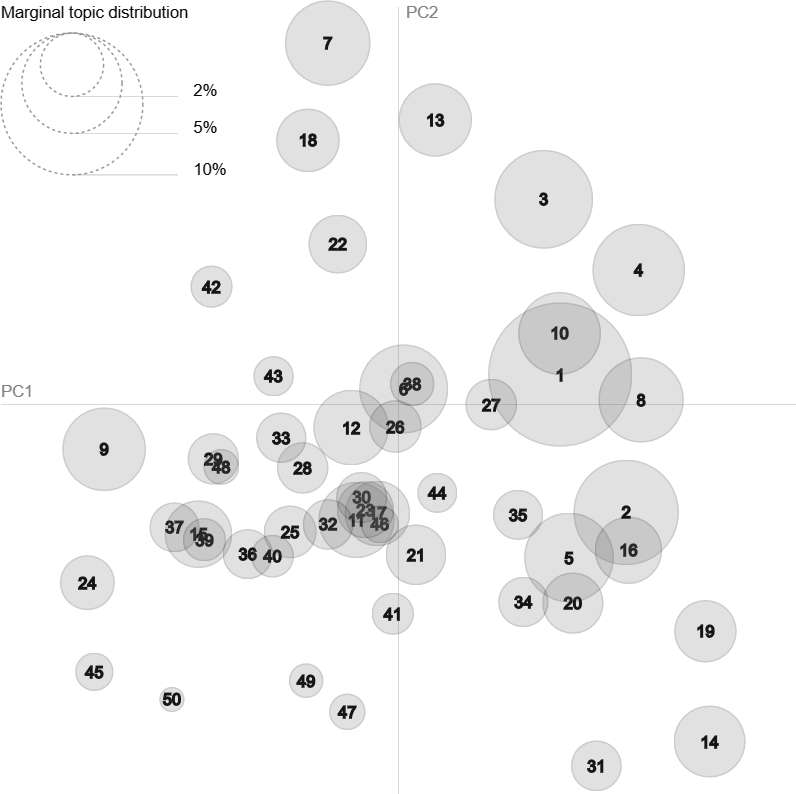
\includegraphics[width=\linewidth]{ldavis-modified}
    \caption{LDAvis applied on \emph{Bitcoin} with $K=50$. The centers of the circles indicate the position of the topic-word distributions after being reduced with \ac{MDS}, the radii display the relative importance of the topic for the entire corpus.}
    \label{fig:ldavis} 
\end{figure}

\subsection{Dimension Reduction}
Given the extracted topics $\phi_1, \dots, \phi_K$ and the document-topic distributions $\theta_1, \dots, \theta_m$, we first project the topic vectors to two dimensions.
We adapt the approach by Sievert et~al. \cite{sievert2014ldavis}, which is given by applying \ac{MDS} to the disimilarity matrix derived from the Jensen-Shannon divergence.
\ac{MDS} yields projections $\bar{\phi}_1, \dots, \bar{\phi}_K$, such that the euclidean distance between projected points reflects the dissimilarity between the high-dimensional points.
A document $d_i$, $ 1\le i\le m$ viewed as $K$-length vector $\theta_i = (\theta_i^{(1)}, \dots, \theta_i^{(K)})$, is then represented by the convex linear combination $\bar{d}$, precisely
\begin{align}
    \bar{d} = \sum \limits_{j=1}^{K} \theta_i^{(j)} \bar{\phi}_j.
\end{align}
A direct application of \ac{MDS} to the document-topic vector as done in \cite{linstead09sourcerer} neglects the similarity of topics to each other as shown in \autoref{fig:ldavis}.

\section{\uppercase{Visualization Approach}}
\label{sec:conceptvisualization}
\noindent 
Since software has no intrinsic gestalt, our visualization must project the properties of the processed topic model data onto graphical primitives. 
This can be done by utilizing its visual variables and either providing an explanation, how the mapping of information to the variables is done, or by making use of metaphors that are known to the users (or both).

\paragraph{Tree Metaphor.} 
Our visualization applies a tree metaphor: each source code unit is represented by an individual tree. 
All source code units together make up the software project and are depicted as a forest.
The trees provide different visual variables that can be utilized, such as their type and height, the size of their trunk and crown, or the amount and color of their leaves.
The position and displayed proximity of two trees allows drawing conclusions about topic similarity easily.
In addition, we can rely on easy-to-understand concepts such as health, age, or season of trees in order to convey common software metrics such as test coverage, change frequency, or size.
Anomalies in the source code files, such as many occurring errors or rapidly changing topics, can be displayed by tree stumps, or fallen or burning trees.

In our prototype, we decided to allow users to choose their own mappings by listing available visual variables and properties of the used source code entities. 
As an example, users can visualize the dominant topic with the tree type, as can be seen in \autoref{fig:example1}, and thus recognize which files contain similar topics.
Users can explore the 3D forest by rotating, pan, and zoom using the virtual camera by means of a world-in-hand navigation.
To reduce rendering cost and maintain visual clarity we opted for simpler, low-poly tree geometries instead of realistic tree rendering---we integrated and experimented with a technique for large scale forest rendering first \cite{bruneton2012real} but found it difficult to increase the visual expressiveness of individual trees. 
The resulting visualization can be categorized as $\mathcal{A}^3 \oplus \mathcal{R}^2$, i.e., three-dimensional graphical primitives on a two-dimensional reference space \cite{duebel2014-2d3drepresentation}.

\begin{figure}[t]
    \centering
    \begin{tikzpicture}[spy using outlines={white, circle, magnification=1.8, size=96, connect spies, every spy on node/.append style={thin}}]
        \node[anchor=center, inner sep=0pt, outer sep=0pt](tooltip) {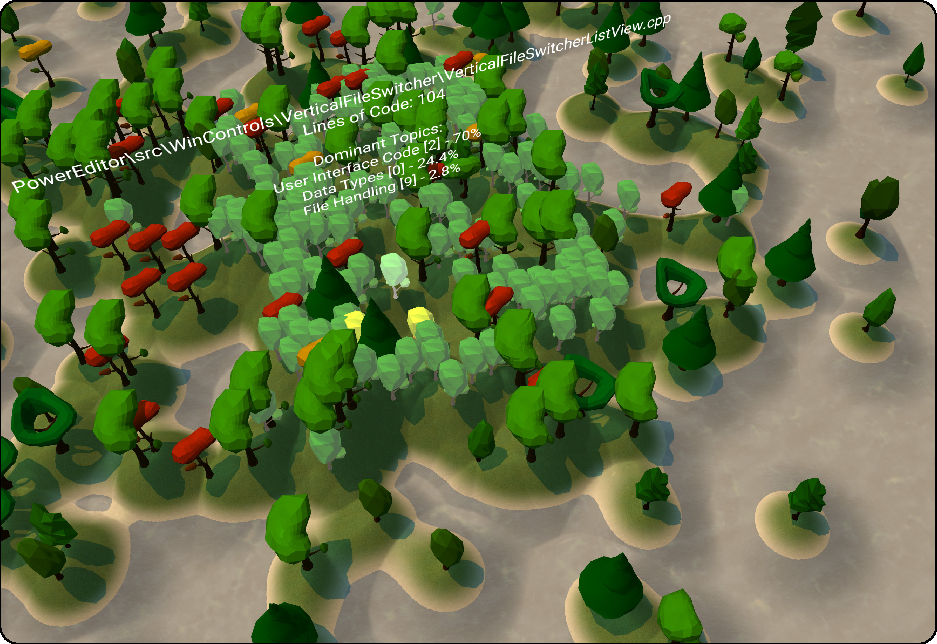
\includegraphics[width=\linewidth]{forest-tooltip.pdf}};%
        \spy on ($(tooltip)+(-0.65, +1.1)$) in node at (+1.85, -0.7);
    \end{tikzpicture}
    \caption{Visualization of the \emph{notepad-plus-plus}\footnotemark~project. The dominant topic of each source code file is visualized with the tree type. The cursor hovers over a light green tree and identical trees, i.e., similar source code files, are highlighted. For the selected tree, information on the corresponding source code file, such as file path, lines of code and its dominant topics, is shown above. 
    In this example, the pre-computed topics have been labeled manually to provide comprehensible topic descriptions.}
    \label{fig:tooltip}
\end{figure}

The visualization is also intended to support software systems of more than \numprint{10000} source code units such as \emph{TensorFlow}.
This raises the issue that the visualization of so many files and thus so many trees can get confusing. 
To alleviate this issue, our visualization emphasizes dense tree clusters by making use of the terrain's height.
Each tree is assigned to a terrain height depending on how many trees can be found in its surroundings and trees in denser clusters then can be found on hills. 
To be able to differentiate various clusters, a water surface with adjustable height can be used to separate different hills from one another. 
Furthermore, users can receive information about each tree via hovering over it.
Depending on the zoom level of the visualization, a tooltip is shown for the hovered tree, containing the name and details of the represented software code file or project, such as software metrics or information about its topic distribution (\autoref{fig:tooltip}).
Trees with the same identical dominant topic are highlighted to emphasize topic clusters.

\begin{figure*}[t]
    \centering
    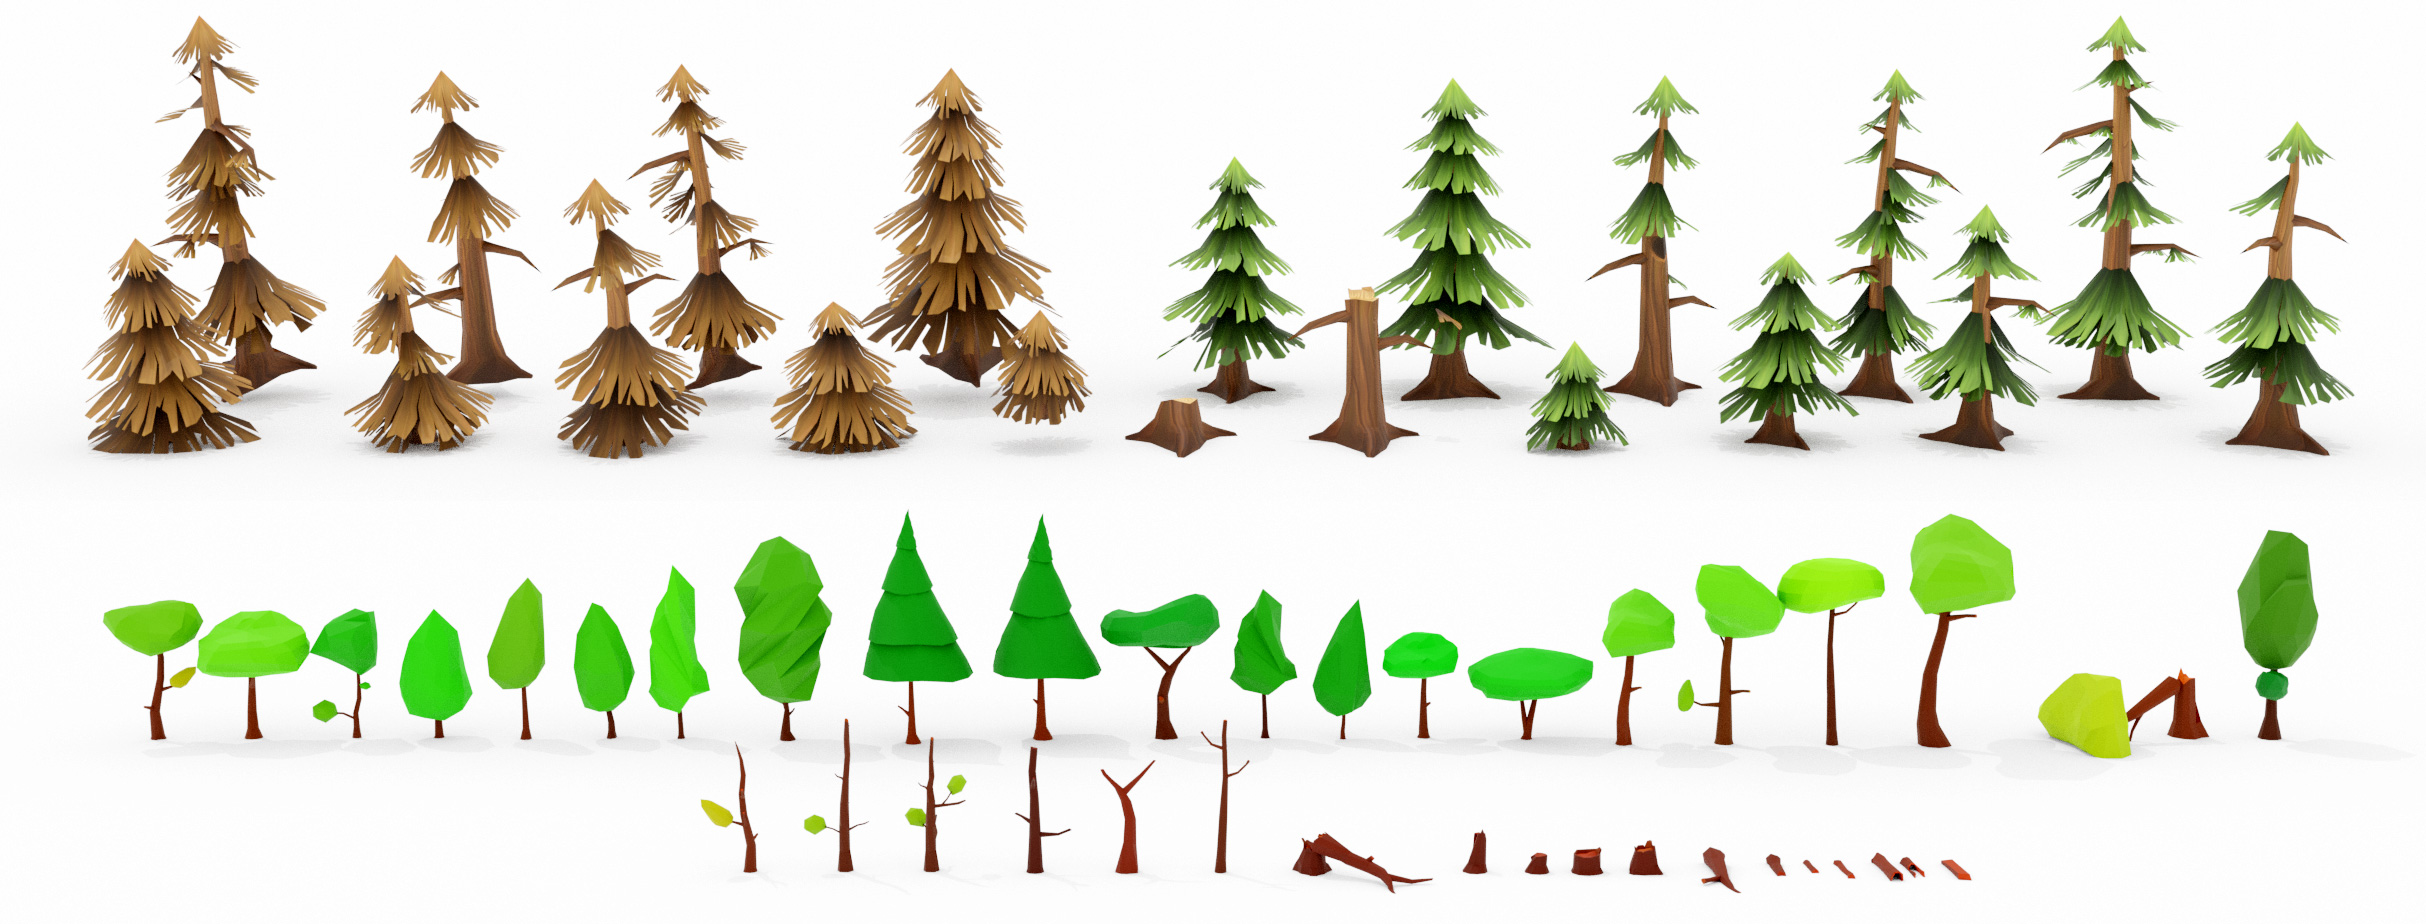
\includegraphics[width=0.9\textwidth]{forest-meshes-hand-painted.jpg}
    \caption{Examples of two handcrafted 3D tree model sets: top row shows a pine tree, modeled and hand painted in various stages, sizes, and health conditions. The bottom row shows low-poly meshes of various tree types in color variation. The models were purchased on Sketchfab: \enquote{HandPainted Pine Pack} by ZugZug and \enquote{Low Poly Nature Pack} by NONE.}
    \label{fig:trees-handpainted}
\end{figure*}

\label{subsec:connectionDataViz:Modelfiles}
\paragraph{Tree Geometry.}
We use handcrafted geometry from Sketchfab, rather than designing our own models or generating geometry dynamically (\autoref{fig:trees-handpainted}).
While the latter approach could introduce numerous variations, handcrafted geometry keeps the visualization framework easily customizable and reduces the overall complexity.
Generating 3D trees at runtime would allow data to be displayed in an arbitrary exact fashion.
However, rendering highly individual meshes increases the complexity for and requirements on web-based implementations.
In contrast, handcrafted models tend to increase the visual quality more and can easily be instanced and rendered.

\footnotetext{\url{https://github.com/notepad-plus-plus/notepad-plus-plus}}

The model files are expected to contain multiple variations of trees using scene-graph semantics.
Furthermore, for every tree, multiple variation of the tree must be associated to a specific combination and range of visual variables and data respectively, e.g., tree growth requires information on which variations represent correspondingly large or small grown trees.

Each model file is stored with a description file that captures each tree variant and its attributes used in the visualization.
Although automatic creation of this description file is imaginable, e.g., through use of heuristics or rule-based approaches, we manually created our description files.
In detail, each description file contains the following information:
Each file contains a list of tree types and variants along with an overview of meta-information about the corresponding model. 
The overview stores a reference to the model file it describes, a list of the identifiers used for all visual variables labeled and information on how to scale the whole scene to create a consistent visualization. 
By storing an explicit reference to the model file, multiple descriptions can be used for a single asset file, e.g., when asset files contain multiple, different 3D models.

The list of distinct variants follows a two-level structure: 
On the top level, models are grouped by their tree type, as this property separates fundamentally different trees. 
Within each tree type, a generic representative is named and a list of tree variants is recorded, e.g., trees of type \enquote{birch} with different growth states. 
Every tree variant assigns concrete manifestations in form of numeric values to each of its visual variables. 
Models in the description file are referenced by their scene identifier from the model file scene graph.
With the description and the model file, data points in the framework can be visualized using its models and all visual variables of the file get shown to the user for attribute mapping.
Users can freely assign data attributes to tree variables, e.g., by assigning the age of a software project to the growth state of the trees.
As each set of models provides only a finite set of tree variants, not every value combination can be expressed directly, especially if multiple visual variables are used. 
We employed a model selection algorithm to choose the most suited tree model for each data point.
To facilitate this, the algorithm rates each tree model based on the difference between encoded values of each of the used variables and their attributes.

\label{subsec:connectionDataViz:CSV}
\paragraph{Data Input.}
The data processing on source code repositories can take anything between hours and days, thus we decoupled data processing and visualization by storing the results in a structured, intermediate data format with the following constraints:
\begin{itemize}
    \item Each data point will be represented by one tree.
    \item Each data point has attributes that represent a 2D position to place the tree in the terrain.
    \item Each data point might have additional attributes, e.g., dominant topics, file name or metrics.
\end{itemize}

\noindent This separation allows for the visualization, to be used with data from topic models as well as any input that complies to these constraints, e.g., data from other domains such as geo-referenced data.

\section{\uppercase{Implementation}}
\label{sec:implementation}
\noindent
The implementation is separated into two distinct component: data processing and visualization.
The interface between both components are structured files where one file represents one data set.
Thereby, the structured data set uses the common CSV file format.
The data processing pipeline and the visualization approach are implemented as follows.

\subsection{Data Processing}
\label{subsec:impldataproc}
\noindent 
We use the Python package environment and the \emph{GitHub API for Python} for gathering our corpus. 
For preprocessing, we use the \emph{nltk}\footnote{\href{https://www.nltk.org/}{https://www.nltk.org/}} and \emph{spacy}\footnote{\href{https://spacy.io/}{https://spacy.io/}} library for lemmatization and obtaining a stop word list for the English language.
One of the bottle necks of our data pipeline is the main memory. 
Large projects like \emph{TensorFlow} may exhaust the main memory especially during lemmatization. 
Therefore, we chose to process projects in batches and process them sequentially, optimizing the preprocessing steps for this kind of distributed computing. 
The results of this step were cached and saved in text files that can be loaded during runtime to avoid redoing this step for a project.

After finishing preprocessing, we used the \emph{gensim}\footnote{\href{https://radimrehurek.com/gensim/}{https://radimrehurek.com/gensim/}} implementation for LDA. 
It provides a convenient optimization pipeline with random search as well as dealing properly with relatively large amounts of data. 
For optimization and the dimension reduction algorithms, we used the \emph{scikit-learn} library\footnote{\href{https://scikit-learn.org/stable/index.html}{https://scikit-learn.org/stable/index.html}}. 

\subsection{Visualization}
\label{subsec:implvis}
\noindent 
The visualization component is implemented as a web-based visualization system that processes the CSV files.
Thereby, the component is implemented using TypeScript and WebGL to be used in modern web browsers. 
As the browser integration and rendering is based in the open-source framework \emph{webgl-operate}\footnote{\href{https://webgl-operate.org}{https://webgl-operate.org}}.
It provides some abstraction in accessing WebGL rendering functions, including some very high-level functionality such as a ready-to-use label rendering pass or glTF\footnote{\url{https://www.khronos.org/gltf/}} scene loading functionality.
On top of this, the terrain and tree rendering functionality are implemented as extension to the framework.

\paragraph{Tree Geometry.}
The visualization component handles 3D models, i.e., the trees, encoded using the glTF file format.
To describe the models contained in the scene graph, a hand-managed description file in JSON format is provided by the visualization designer, associating visual variables with a number 3D models in the scene graph.
Each tree model is represented by a scene graph node within the while glTF file.
Since trees may inherit a translation in the scene graph, the translation is normalized and adjusted to the tree position in the terrain for this visualization.
Each tree has a corresponding data structure in memory and on the GPU as vertex buffers that contains all its attributes, given through the current attribute mapping.
When the mapping changes, i.e., the user selects a different CSV column for a tree attribute, the attributes are updated and the vertex buffers are updated accordingly.
After a change in its attributes, the tree model for a data point is determined by a best-fit approach among the rule set of the description file.

\paragraph{Terrain Generation.} 
When loading a data set, the terrain is calculated based on the tree density.
For this, the terrain is subdivided into a grid with a fixed resolution.
For each tree, a Gaussian kernel is applied at its position, increasing the terrain height there and in the vicinity.
In cases where many trees are next to few trees, the height is flattened with a non-linear fall-off, resulting in a flatter, more plain terrain.
The goal is that the densest cluster on the whole terrain will reach maximum terrain height while a single tree will still have a clearly visible terrain height of ca. 30-50\% of the maximum terrain height.
In addition to the hills and beaches of the terrain, a static water texture is rendered to give a sense of cohesion to clustered tree groups.
The water level is configurable in the user interface and may be used for height-filtering of data points \cite{limberger2018-reference}.

\begin{figure*}[t]
    \centering
    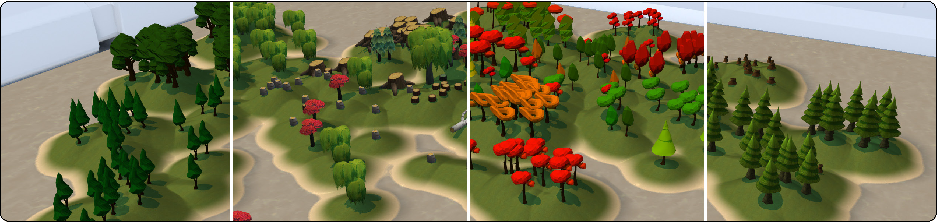
\includegraphics[width=\textwidth]{forest-variants.pdf}
    \caption{Four different assets comprised of different tree geometries and styles used for data mapping. 
    The mapping, the number of visual variables, and the overall expressiveness of the forest is highly dependent on the assets and its description.}
    \label{fig:trees-variants}
\end{figure*}

\paragraph{Tree Placement.}
Stating no additional assumptions on the characteristics of the 2D layout of the data processing pipeline, data points in the 2D layout may overlap or may be positioned very close to each other.
Since the tree models have an actual and visible volume, these positions are not directly suitable for a clear visualization and may lead to trees standing within another.
In order to prevent this, a basic collision reduction algorithm is applied.
First, the terrain is subdivided into a grid with a fixed resolution.
Then, each tree is assigned the closest position on this grid.
If the closest position is already taken, alternative positions in the vicinity are checked until a free position is found.
The alternative positions are looked up based on a fixed circle kernel in a clockwise direction, incrementally increasing the radius until the search kernel is exhausted.
In order to not make the clusters seems artificial because of the introduced circle-like structures, a random offset based on the original position is introduced. 
This results in the natural looking clusters in comparison to sole square or circle kernels.

\paragraph{Rendering.}
The tree rendering itself is implemented using {WebGL 2} and its instanced rendering capabilities, i.e., the \texttt{drawElementsInstanced()} API.
This makes it possible to efficiently render a model multiple times in the scene and allows to depict a large number of data points.
However, tree types and their visual variables might change dynamically, thus, it is necessary to adjust the buffers sent to the GPU frequently since each tree might change its visual representation on every change in the attribute mapping.

\section{\uppercase{Results \& Discussion}}
\label{sec:results}

\begin{figure}[b]
    \centering
    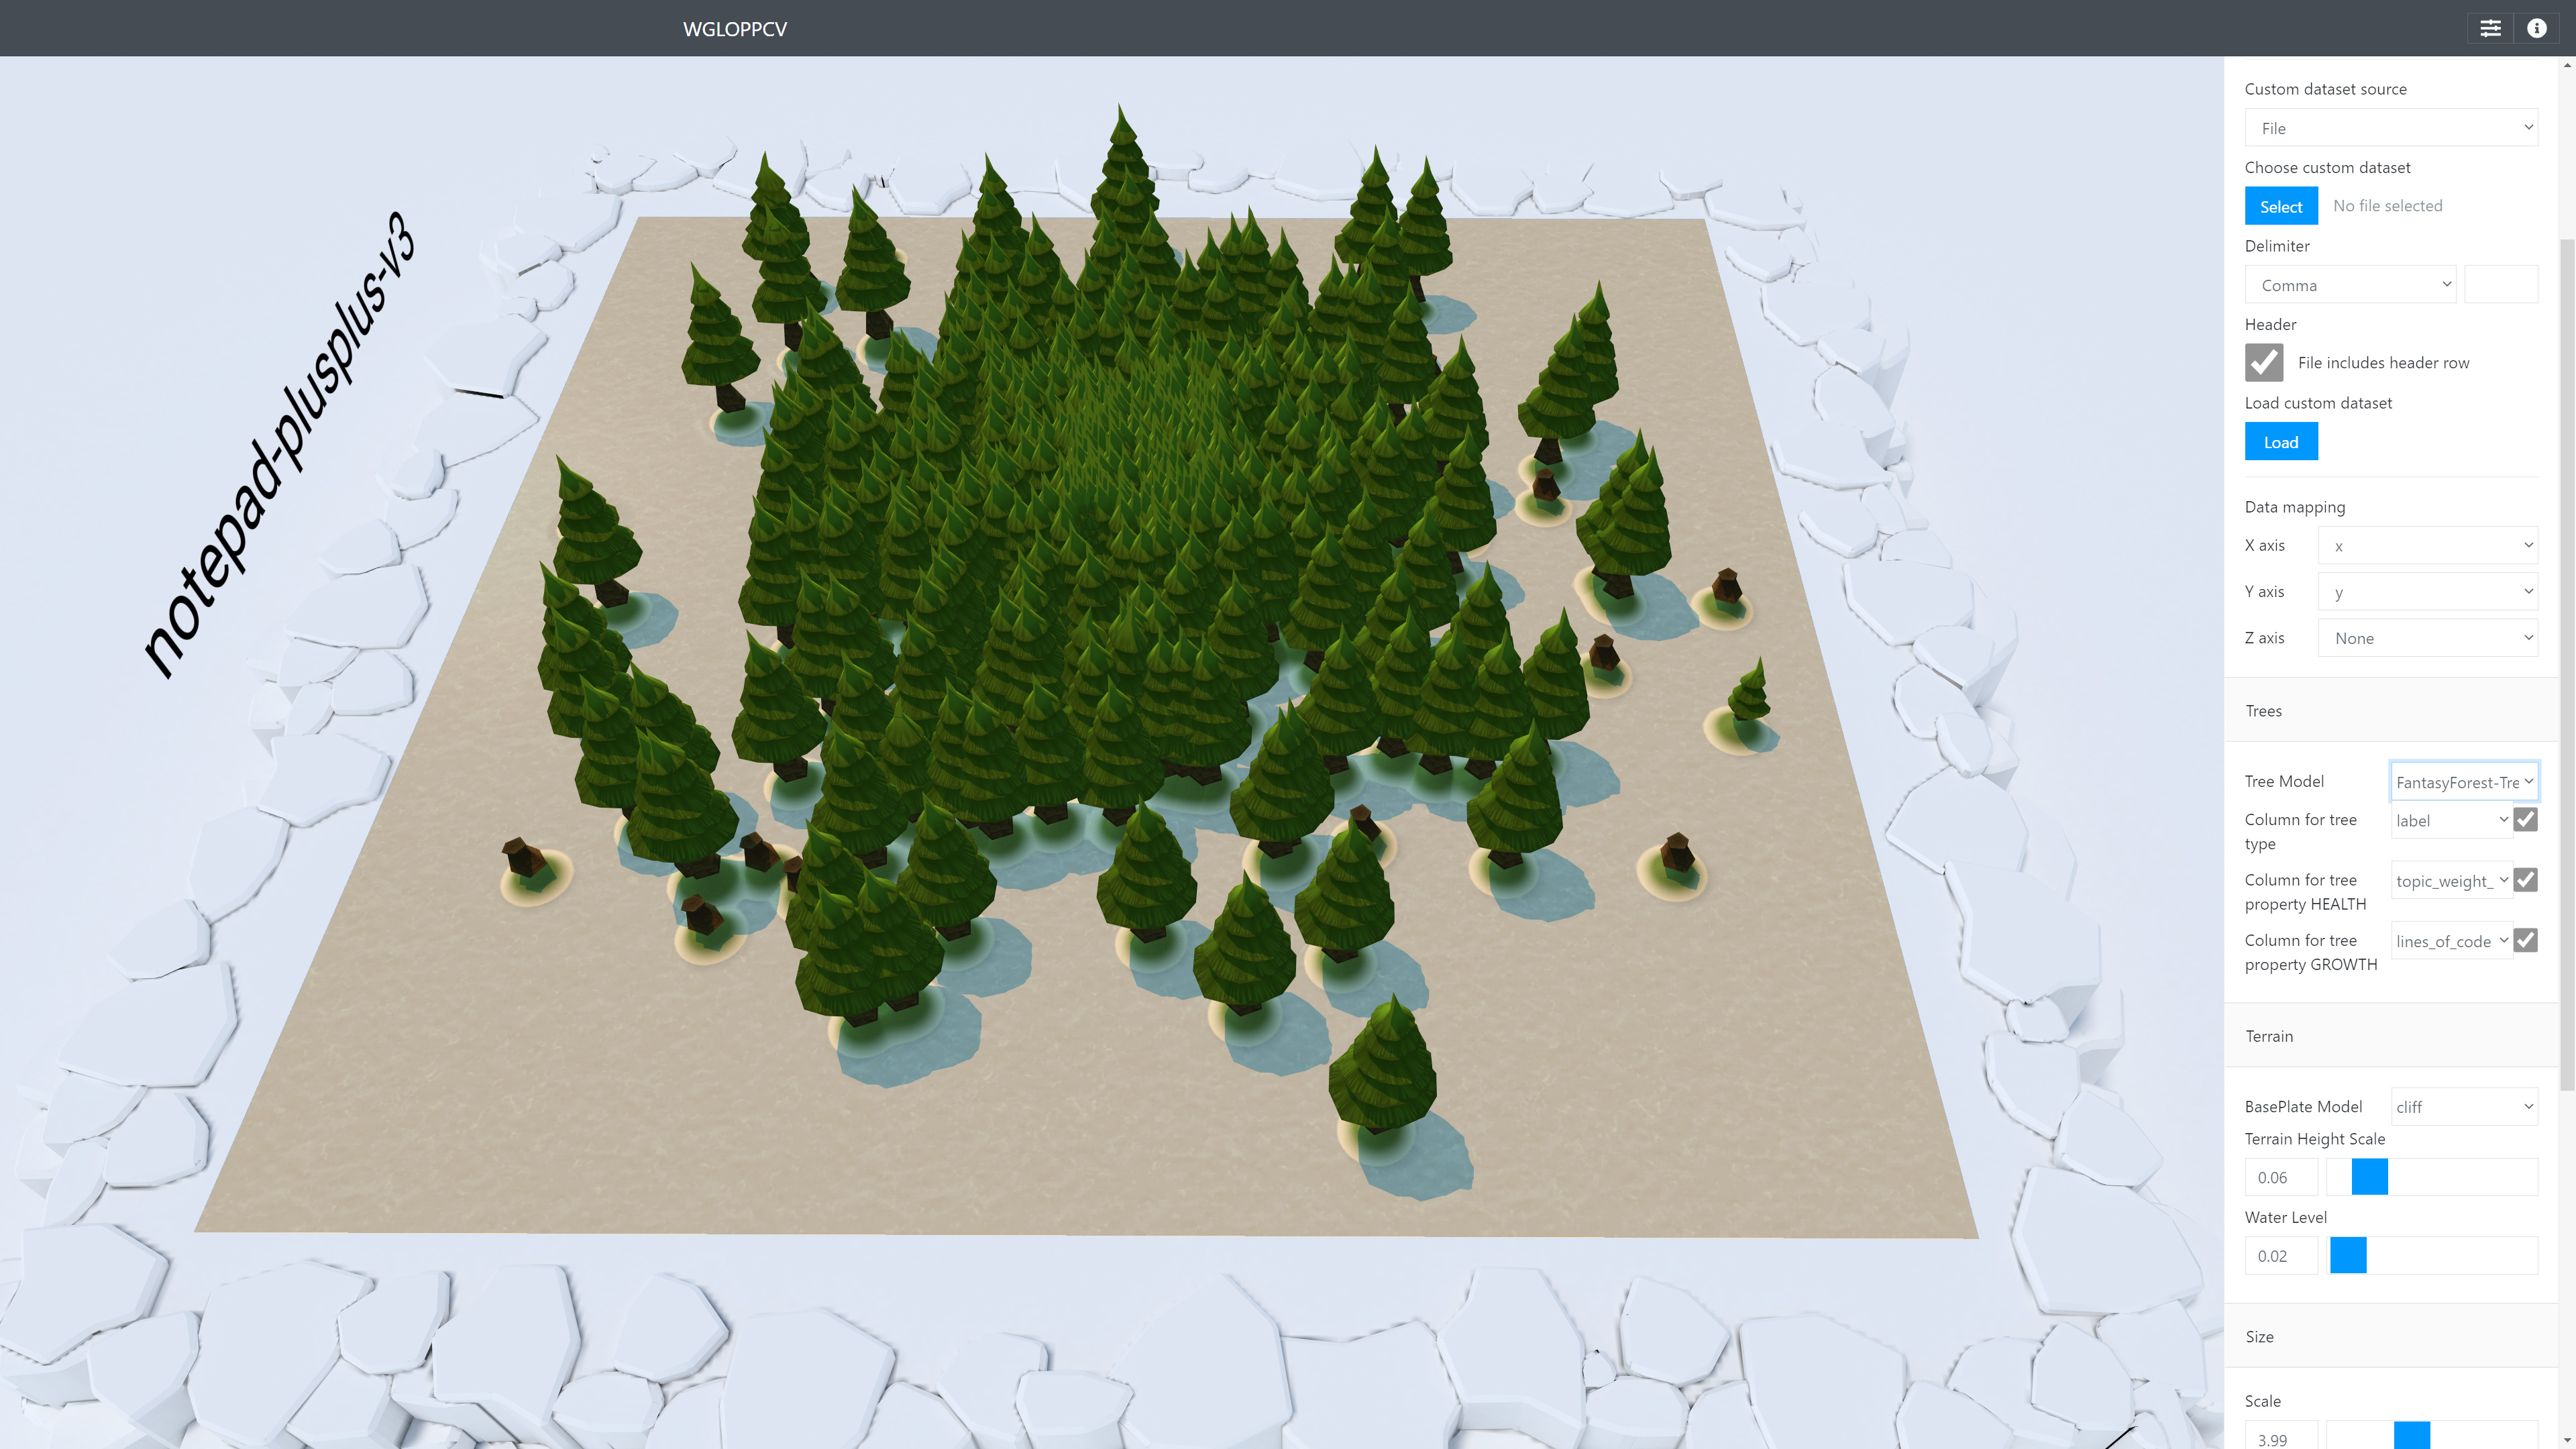
\includegraphics[width=\columnwidth]{forest-gui}
    \caption{GUI of our visualization running in a browser.}
    \label{fig:trees-gui}
\end{figure}

\noindent 
We built a renderer that runs in modern web browsers and can thus be used on a variety of desktop and mobile devices (\autoref{fig:trees-gui}).
Moderately sized software projects ($>$\numprint{10000} entities) can be explored interactively with an integrated graphics chip. 
With a dedicated graphics card, even bigger projects ($>$\numprint{100000} entities) can be visualized with interactive frame rates. 
In the visualization, different presets are available that store a configuration for the major user interface options and can be used to get a first impression of the framework or to get a similar view on different data sets quickly. 
Apart from that, every option can be adjusted to customize the visualization: 
The data sets can be chosen from a list of uploaded data sets or own data sets can be uploaded.
Additionally, the currently used model files can be changed during runtime.
The available visual variables of the model file are displayed in the user interface and can be assigned to data attributes.
The set of example use cases shown in this work underline the capabilities of the proposed framework but are not hard-wired in the structure of the framework. 
Instead it is possible to easily adjust the visualization for other needs if the constraints on the data format are met, custom data files can be used and visualized.

\subsection{Examples}
\label{subsec:examples}
\noindent
Apart from the currently provided assets and their descriptions, other glTF scenes can be used to visualize the provided data (\autoref{fig:trees-variants}).
This effectively means swapping trees with other objects and provide appropriate visual variables, e.g., buildings, street furniture, rocks, flowers, etc.
The listing~\ref{lst:basic2d} shows an excerpt of the description file used for \autoref{fig:teaser}.
\begin{lstfloat}[b]
    \lstinputlisting[language=TypeScript]{listings/biome-trees-excerpt.json} 
    \caption{JSON configuration of a mapping from attribute values to 3D model.}
    \label{lst:basic2d}
\end{lstfloat}
\autoref{fig:notepad} shows a forest of the \emph{notepad-plus-plus} project.
The resulting topics of the software files are mapped to tree types and 2D position.
A cohesive cluster in the center made up of tall, light green trees can be recognized.
When inspecting the trees of this cluster using the mouse cursor, tooltips reveal that they share a dominant topic.
Analyzing the words this topic comprises, the files can be related to user interface code.
The topic model is correct in this judgment since the files displayed in this cluster indeed deal with the user interface of \emph{notepad++}.
\begin{figure}[t]
    \centering
    \begin{tikzpicture}[spy using outlines={white, circle, magnification=2.5, size=80, connect spies, every spy on node/.append style={thin}}]
        \node[anchor=center, inner sep=0pt, outer sep=0pt](notepad) {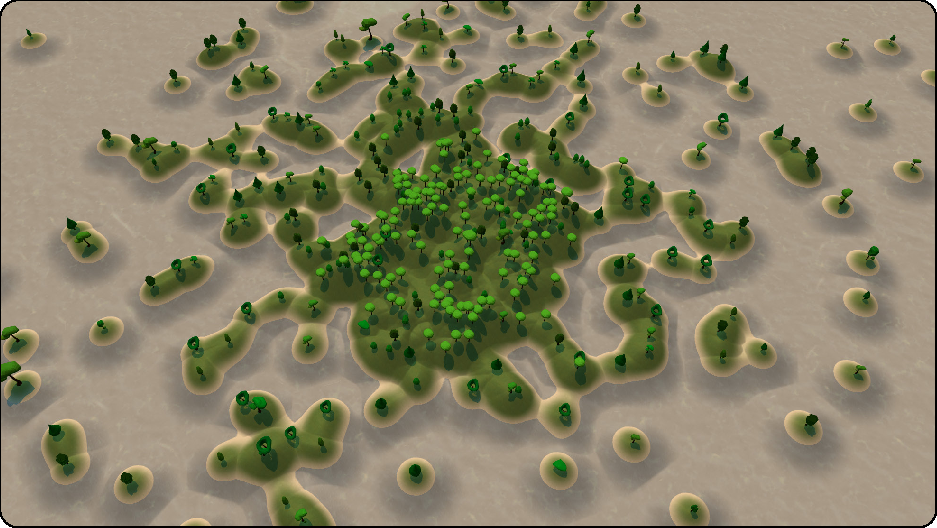
\includegraphics[width=\columnwidth]{forest-notepad.pdf}};%
        \spy on ($(notepad)+(-0.5, +0.0)$) in node at (+2.2, +0.0);
    \end{tikzpicture}
    \caption{Software forest of \emph{notepad-plus-plus} project.}
    \label{fig:notepad}
\end{figure} 

In \autoref{fig:software40}, 40 different open-source projects are visualized.
The projects have been processed and their topic weights have been determined.
The \emph{Software Forest} allows to recognize similar projects, e.g., deep learning projects.
The cluster of red maple trees is composed of deep learning projects such as \emph{CNTK}, \emph{caffe}, \emph{Pytorch}, and others.

\subsection{Limitations}
\label{subsec:limitations}
\noindent 
For now, we manually labeled the topics in order to give more context to users beyond the numerical topic index and word vectors. 
Since the topics returned by LDA are latent, they have no inherit label mechanism \cite{blei2003latent}. 
This labeling is an essential part for making our visualization interpretable. 
Therefore, efficient ways to label topics automatically and consistently should be researched, also drawing from previous work and literature about this known problem of latent topic modeling \cite{magatti2009automatic}.

The proposed work could benefit from the usage of more data sources. 
Similar to Linstead et~al. bug reports could be considered for additional input as well \cite{linstead2007mining}. 
We did some first experiments using so called joint embeddings \cite{yu2017joint}, which can be used for the integration of more diverse data sources, but more work needs to be done to conclude whether or not this is a promising approach.

When exploring large projects, dense clusters of trees occur frequently.
To improve the visual clarity of the system, it would be possible to recognize clusters and aggregate similar trees in the visualization.
Hovering over these trees or zooming into their region, the trees clusters could be expanded again, or tooltips with additional details could be shown.

\begin{figure}[t]
    \centering
    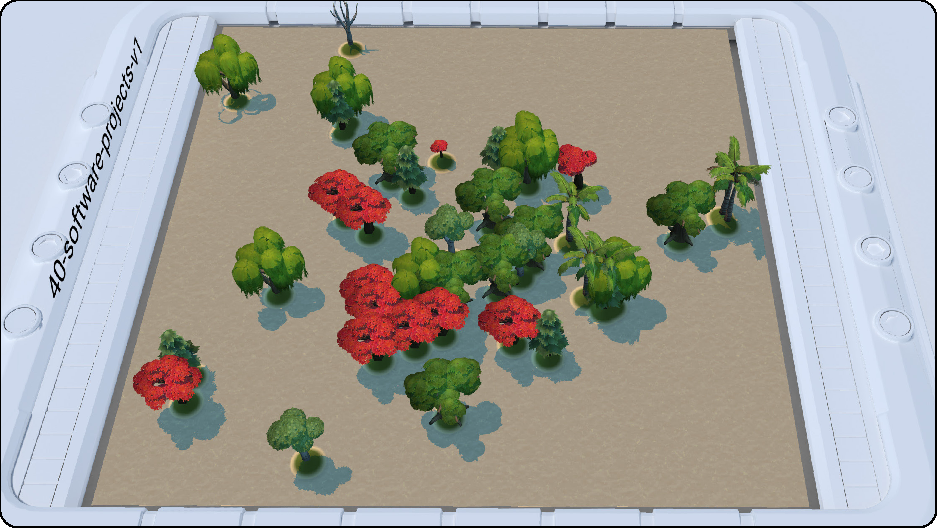
\includegraphics[width=\columnwidth]{forest-software40.pdf}
    \caption{Software forest of 40 open-source projects.}
    \label{fig:software40}
\end{figure}

\section{\uppercase{Conclusions}}
\label{sec:conclusion}
\noindent
The approach to visualize software data, i.e., a prominent example of data without intrinsic gestalt, using metaphors is often-tried but only scarcely used outside of research communities.
We try to address application issues by proposing a metaphor close to nature and a dedicated visualization approach.
As such, we propose \emph{Software Forest}, a novel 2.5D software visualization to interactively explore a software system illustrated as a forest.
The visual metaphor allows for multiple visual variables, including, but not limited to, tree type, growth state, height, and color.
The layout of the forest is derived from a source code document analysis using Latent Dirichlet Allocation and Multidimensional Scaling.
This layout reflects similarity in semantics of source code by proximity, and, thus, allows for an alternative mapping and view than traditional software visualization approaches such as treemaps.
The layout is used for deriving a terrain and locations for the trees for further attribute mapping.
The rendering approach takes different parameterization, different visual variables, and scalability into account.
As such, using different 3D models is feasible and requires only the composition of a glTF scene graph and a description file with information on individual models and specific attribute mapping.
The approach is exemplified using mid-sized open-source software development projects.
An application to the data sets indicates both an effective layout base on semantic similarity of source code and an explorative visualization approach of the resulting maps.

\par
Future work can be discussed separately for layout generation and the visualization approach.
For layout improvements, software similarity \cite{almsiedeen2013-similarity} and suitable dimensionality reduction methods \cite{cha2007comprehensive,vernier2020-reduction} are target for further research.
The visualization approach needs to be evaluated regarding readability using user studies.
Regarding variability of the 3D models, tooling on the glTF models would simplify the integration of other 3D models, even for applications outside of forest metaphors.
As the input for the prototypical viewer are CSV files with explicit layout and additional attributes as columns, we already imagine easy visualization prototyping and adaption in other visualization domains as well.
Using a broader perspective, the proposed visualization approach allows for visualization of structured data sets with scatter-plot layout and dynamic model mapping for a wide-spread use of thematic mapping -- the topic maps.

\section*{\uppercase{Acknowledgements}}
\label{sec:acknowledgements}
\noindent
We want to thank the anonymous reviewers for their valuable comments and suggestions to improve this article.
Further, this work is part of the \enquote{Software-DNA} project, which is funded by the
European Regional Development Fund (ERDF -- or EFRE in German) and the
State of Brandenburg (ILB) as well as the \enquote{TASAM} project, which is funded by the German Federal Ministry for Economic Affairs and Energy (BMWi, ZIM).

\bibliographystyle{apalike}
{\small
\bibliography{example}}

\begin{acronym}
\acro{AST}{Abstract Syntax Tree}
\acro{ATM}{Author-Topic Model}
\acro{DTM}{Developer-Topic Model}
\acro{LDA}{Latent Dirichlet Allocation}
\acro{LSI}{Latent Semantic Indexing}
\acro{LOC}{Lines-of-Code}
\acro{NLP}{Natural Language Processing}
\acro{MBTI}{Myers-Briggs Type Indicator}
\acro{MDS}{Multidimensional Scaling}
\acro{MTM}{Multi-feature Topic Model}
\acro{SE}{Software Engineering}
\acro{BOW}{Bag-of-Words}
\acro{TTM}{Tag-Topic Model}
\acro{VCS}{Version Control System}
\end{acronym}

\end{document}
